% Homotopy of paths
% Author: Alain Matthes
% https://creativecommons.org/licenses/by/2.5/
\documentclass[a4paper,10pt]{article}
\usepackage{tikz}
\usetikzlibrary{arrows,calc,shapes,decorations.pathreplacing}
\begin{document}
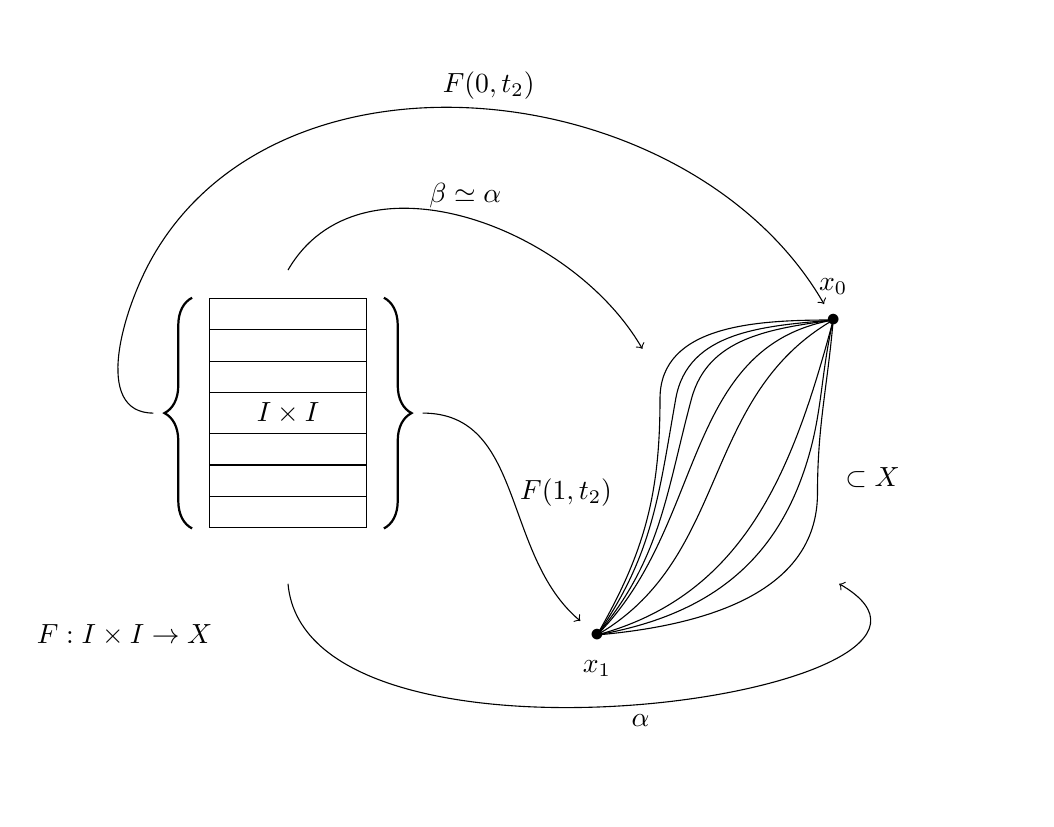
\begin{tikzpicture}
  \node at (0,0) {$F : I \times I \rightarrow X$};
  \node[label=below:$x_1$]  (x1) at (6,0)  {$\bullet$};
  \node[label=above:$x_0$]  (x0) at (9,4)  {$\bullet$};  
  \node  at (9.5,2)  {$\subset X$}; 
  \draw (x1.center) to [out=5,in=-90]++(2.8,1.8) to[out=90,in=-95](x0.center);
  \draw (x1.center) to [out=10,in=-110]++(2.6,2) to[out=70,in=-103](x0.center); 
  \draw (x1.center) to [out=15,in=-105](x0.center);
  \draw (x1.center) to [out=30,in=-150](x0.center);
  \draw (x1.center) to [out=45,in=-170](x0.center); 
  \draw (x1.center) to [out=50,in=-105]++(1.2,3)to [out=75,in=-172](x0.center); 
  \draw (x1.center) to [out=55,in=-100]++(1.0,3) to[out=80,in=-175](x0.center); 
  \draw (x1.center) to [out=60,in=-90]++(0.8,3) to[out=90,in=-180] (x0.center);
  \begin{scope}[every node/.style={draw, anchor=text, rectangle split,
    rectangle split parts=7,minimum width=2cm}]
    \node (R) at (2,4){ \nodepart{two} \nodepart{three}
    \nodepart{four}$I\times I$\nodepart{five}\nodepart{six}\nodepart{seven}};
  \end{scope}
  \draw[decorate,decoration={brace,mirror,raise=6pt,amplitude=10pt}, thick]
    (R.north west)--(R.south west) ;
  \draw[decorate,decoration={brace,raise=6pt,amplitude=10pt}, thick]
    (R.north east)--(R.south east); 
  \draw[->] ($(R.west)+(-20pt,0)$) to[out=-180,in=240] ++(0,2)
    to [out=60,in=120]node[above,midway]{$F(0,t_2)$}(x0) ; 
  \draw[->] ($(R.north)+(0,10pt)$) to [out=60,in=120]
    node[above,midway]{$\beta \simeq \alpha$} ++(4.5,-1) ; 
  \draw[->] ($(R.east)+(20pt,0)$)  to [out=0,in=140]
    node[right,midway]{$F(1,t_2)$}(x1) ; 
  \draw[->] ($(R.south)+(0,-20pt)$)  to [out=-85,in=-30]
    node[below,midway]{$\alpha$}++(7,0) ;    
\end{tikzpicture}
\end{document}
